\documentclass[man,12pt,a4paper]{apa6}

\usepackage[utf8]{inputenc}
\usepackage[ngerman]{babel}
\usepackage{amsmath}
%\usepackage[onehalfspacing]{setspace}
\usepackage[style=apa,sortcites=true,sorting=nyt,backend=biber]{biblatex}
\usepackage{pdfpages}

\DeclareLanguageMapping{ngerman}{ngerman-apa}
\addbibresource{literatur.bib}

\title{Seminarstunde zum problemorientierten Unterricht}
\shorttitle{Problemorientierter Unterricht}
\author{Stephan Kulla}
\leftheader{Kulla}
\affiliation{TU München}

\begin{document}
% https://tex.stackexchange.com/a/283463
\thispagestyle{otherpage}

\maketitle

\section{Problemorientierter Unterricht}

\subsection{Wozu problemorientierter Unterricht?}

Die Digitalisierung wird weitreichende Folgen und Auswirkungen auf die zukünftige Arbeitswelt haben \parencite{dengler2015}. Wenn man beispielsweise der Studie von \textcite{frey2017} folgt, so könnte in den USA in den nächsten 20 Jahren jeder zweite Job durch die Arbeit von Computer ersetzt werden. \textcite{dengler2015} schätzen in ihrem Bericht, dass $15\%$ der Arbeitsplätze in Deutschland sehr wahrscheinlich durch die Einführung von Programmen wegfallen werden.

Damit stellt sich die Frage an Lehrkräfte, wie sie ihre Schülerinnen und Schüler auf die neue Arbeitswelt vorbereiten können. So argumentiert Günter Dueck, dass das Bildungssystem neue Kompetenzen fördern muss: Soziale Kompetent, Kommunikationsfähigkeit, Problemlösefähigkeit und fachliche Kompetenzen sind einige der vielen Fähigkeiten (Wort?), die in der zukünftigen Arbeitswelt benötigt werden (Zitat).

Problemorientierter Unterricht ist ein forgeschlagener Weg, um diese Kompetenzen bei Schülerinnen und Schülern zu fördern \parencite{silver2004}. Es ist „Unterricht im Geist des Problemlösens“, wie \textcite{reusser2005} es beschreibt. Schülerinnen und Schülern wird ein komplexes Problem präsentiert, welches sie eigenständig (oft in Gruppenarbeit) lösen \parencite{silver2004}. Die Probleme sind dabei lebensnah und authentisch \parencite{kunter2013} oder didaktisch ansprechend aufbereitet \parencite{reusser2005}.

Problemorientierter Unterricht verfolgt das Ziel, transfährfähiges Wissen aufzubauen und fachspezifische Denk- und Lernstrategien zu fördern \parencite{reusser2005}. Durch Gruppenarbeit können außerdem die sozialen und kommunikativen Kompetenzen gestärkt werden \parencite{seidel2014}. Dabei kann problemorientierter Unterricht sowohl eingesetzt werden, um bereits erworbenes Wissen anzuwenden, als auch um neues Wissen zu erwerben \parencite{reusser2005}.

\subsection{Entdeckendes Lernen und Stationenarbeit}

Entdeckendes Lernen und Stationenarbeit sind zwei konkrete Methoden, wie Probleme von den Schülerinnen und Schülern im Unterricht gelöst werden können \parencite{kunter2013}. Bei der Methode des entdeckenden Lernens wird nach \textcite{hameyer2008} wird in der Konfrontationsphase zunächst ein Problem präsentiert. Dieses wird in der Entdeckungsphase von den Schülerinnen und Schüler bearbeitet, wobei die Lehrkraft unterstützend tätig wird. Zum Abschluss werden in der Präsentationsphase die Ergebnisse vor der Klasse präsentiert und diskutiert.

Die Stationenarbeit (auch „Arbeit im Lernzirkel“ oder „Lernen an Stationen“ genannt) ist eine weitere Unterrichtsmethode, um problembasierten Unterricht umzusetzen \parencite{hegele2008}. Nach \textcite{hegele2008} kann diese Form des Unterrichts in fünf Phasen vollzogen werden:

\begin{APAenumerate}
  \item \emph{Hinführung:} Durch Präsentation des Problems soll das Interesse der Schülerinnen und Schüler geweckt werden.
  \item \emph{Rundgang:} Die Lehrerin bzw. der Lehrer stellt alle Stationen vor und gibt Hinweise, die nicht direkt aus den Arbeitsaufträgen ersichtlich sind. Auch auf Gefahren bei der Benutzung von Geräten oder auf vereinbarte Verhaltensweise kann hingewiesen werden.
  \item \emph{Arbeit an den Stationen:} Die Schülerinnen und Schüler arbeiten eigenständig oder in Gruppen an den Stationen.
  \item \emph{Zwischen- oder Schlusskreis:} Abschließende Gespräche zwischen den Arbeitsphasen, um Lernergebnisse zur Kenntnis zu nehmen, das Bewusstsein zu stärken, Teil einer größeren Lerngruppe zu sein oder Lernschwierigkeiten anzusprechen.
  \item \emph{Präsentation der Ergebnisse:} Abschließende Präsentation der Ergebnisse (beispielsweise auf Elternabende, im Klassenzimmer, etc.)
\end{APAenumerate}

\subsection{Forschungsergebnisse}

Pädagoginnen und Pädagogen verknüpften mit der Methode des problemorientieren Unterrichts hohe Erwartungen bezüglich der erzielbaren Lernergebnisse und -motivation \parencite{kunter2013}. Jedoch kommt die Forschung zu gemischten Ergebnissen. Im Vergleich zu rein lehrerzentrierten Unterrichtsänsätzen konnte \textcite{furtak2012} in einer Meta-Analyse mittlere Effekte bei den Lernergebnissen mit der Methode des entdeckenden Lernens nachweisen. Die durchschnittliche Effektstärke wird mit $d=0.5$ angegeben. Jedoch zeigte sich mit $\sigma = 0.56$ eine hohe Standardabweichung in den berichteten Effektstärken der betrachteten Studien. Die Effekte sind jedoch besonders dann hoch, wenn die Schülerinnen und Schüler ihre Forschungsaktivitäten reflektieren müssen bzw. ihre Befunde einordnen müssen.

Auch ist es wichtig, dass die Schülerinnen und Schüler bei problemorientierten Aufgabenstellungen nicht überfordert werden \parencite{kunter2013}. Problemorientierte Formen des Unterrichts stellen nämlich hohe Anforderungen die Lernenden. Dementsprechend müssen die motivationalen und kognitiven Voraussetzungen der Schülerinnen bei der Plannung solcher Unterrichtssequenzen beachtet werden \parencite{kunter2013}. Eine zu starke schülerzentrierte Ausrichtung mit wenig Rückmeldungen der Lehrkraft kann sich negativ aus die Lernergebnisse auswirken \parencite{kunter2013}. Dies zeigt sich auch in Studien: Problemorientierter Unterricht ist eher dann effektiv, wenn Lehrkräfte einzelne Lernaktivitäten anleitet und begleitet \parencite{furtak2012}.

\section{Planung einer Seminarstunde zum problemorientierten Unterricht}

\subsection{Ziel der Seminarstunde}

Unser Ziel in der Seminarstunde ist es, eine Einführung in das Thema des problemorientierenten Unterrichts zu geben. Die Studierenden sollen wiedergeben können, was problemorientierter Unterricht ist und wie durch Stationenarbeit problemorientierter Unterricht umgesetzt werden kann.

Uns ist besonders wichtig, dass die Studierenden folgende Forschungsergebnisse zu problemorientierten Unterricht kennen und für in ihrem Schuldienst beachten:

\begin{APAitemize}
  \item Entdeckendes Lernen ist eine effektive Unterrichtsmethode \parencite{furtak2012}.
  \item Bei der Unterrichtsmethode des problemorientierten Lernens ist es wichtig, dass der Lernende nicht überfordert wird und ausreichend von der Lehrkraft unterstützt wird \parencite{kunter2013}. Entdeckendes Lernen mit lehrerzentrierten Aktivitäten erzielt bessere Ergebnisse als rein schülerzentrierte Formen \parencite{furtak2012}.
\end{APAitemize}

\subsection{Einleitung (10min)}

Bei der Gestaltung der Seminarstunde orientieren wir uns an das AVIVA-Schema \parencite{aviva}. Zunächst stellen wir kurz mündlich das Thema der Seminarstunde vor (Phase „Ankommen und Einstimmen“). Hinterher aktivierten wir das Vorwissen der Studierenden, indem sie allein oder zusammen mit dem Sitznachbarn / der Sitznachbarin Assoziationen rund um das Thema „problemorientierter Unterricht“ brainstormen sollten. Diese wurden hinterher gemeinschaftlich in einer Mind Map zusammengefasst.

Hinterher wird die Mindmap von uns um wesentliche Aspekte ergänzt. Dabei gehen wir im Speziellen auch auf die Unterrichtsmethode des entdeckenden Lernens nach \textcite{hameyer2008} ein, damit die Studierenden eine Vorstellung bekommen, wie solche Unterrichtsformen aussehen. Im AVIVA-Schema entspricht diese Sequenz der Phase des Informierens.

\subsection{Hauptteil (30min)}

Die besondere Herausforderung besteht darin, dass die Studierenden erst in 3-4 Jahren ihren Schuldienst beginnen werden. Zwar haben sie vorher ein Praktikum an der Schule, wir können aber nicht garantieren, dass sie dabei bereits Erfahrungen mit problemorientierten Formen des Unterrichts machen werden. Wir mussten also die Seminarstunde so gestalten, dass sich die Studierenden noch in vier Jahren an die wesentlichen Ergebnisse der Forschung erinnern werden. Wir haben uns deswegen entschieden, dass die Studierenden selbst spüren können, wie das Maß der Unterstützung die Motivation beeinflussen kann.

Hierzu haben wir die Studierenden in zwei Gruppen aufgeteilt. Beide haben eine ähnliche Aufgabe, bekommen jedoch ein unterschiedliches Maß an Unterstützung. Die eine Gruppe soll vollkommen auf sich gestellt sein. Sie hat die Aufgabe, die wesentlichen Forschungsergebnisse zu problemorientierten Unterrichtsmethoden zu recherchieren und auf Grundlage dieser eine Unterrichtssequenz zur Addition von Brüchen zu entwickeln, die problemorientiert gestaltet sein soll. Die Aufgabe ist bewusst so konzipiert, dass sie die Studierenden überfordert und in den 10 Minuten Gruppenarbeitszeit nicht zu schaffen ist. Als Recherchewerkzeug erhalten sie einen Laptop mit Internetzugang und damit viele potentielle Ablenkungsmöglichkeiten.

Die andere Gruppe soll nur die Unterrichtssequenz zur Addition von Brüchen erarbeiten. Auf einem Blatt, welches jeder Studierende erhielt, wurden bereits die wesentlichen Forschungsergebnisse zum entdeckenden Lernen sowie fachdidaktische Empfehlungen für das Vermitteln der Bruchaddition zusammengefasst. Diese Zusammenfassung haben wir bewusst kurz gefasst, um eine Überforderung zu vermeiden. Auch wird am Anfang der Gruppenarbeitsphase das Arbeitsblatt durch einen der Seminarleiter bzw. -leiterinnen kurz vorgestellt. Die Gruppe soll weitestgehend autonom arbeiten, bei Bedarf soll sie aber Unterstützung bekommen.

Diese Gruppenarbeitsphase wird dabei zusätzlich als Stationenarbeit vorgestellt. Zum einen werden die Studierenden so mit dieser Unterrichtsmethode bekannt gemacht. Zum anderen können sich die Studierenden damit das unterschiedliche Setting der beiden Gruppen erklären, so dass die Wahrscheinlichkeit von frühen Nachfragen vermindert werden. Aus Zeitgründen wird auf einer Präsentation der Ergebnisse verzichtet.

Nach dieser Gruppenarbeitsphase findet eine Umfrage statt. Hier sollen die Studierenden ihre Motivation während der Gruppenarbeitsphase reflektieren. Dabei werden die Gruppen getrennt gefragt. Zum Einsatz kommen Items, die aus der Erfassung des Flow-Erlebens nach \textcite{fks} entlehnt sind. Hier beurteilen Studierende Aussagen wie „Ich war ganz vertieft in das, was ich gemacht habe.“ auf einer 7-stufigen Likertskala, wie sehr diese auf sie zutrifft.

Hinterher wird der Sinn der Gruppenarbeitsphase mit den unterschiedlichen Unterstützungsstrukturen offenbart. Wenn alles gut geht, unterscheiden sich die Gruppen in ihrer Motivation. In diesem Fall sollen die Studierenden selbst reflektieren, was der Grund dafür ist. Hier sollen die Studierenden die fehlende Unterstützung als Hauptgrund identifizieren. Sollte die Umfrage nicht dem erwarteten Ergebnis entsprechen oder die Studierenden andere als die erwarteten Gründe nennen, stellen wir die Idee hinter der Umfrage und Gruppenarbeitsphase vor. Gegebenfalls diskutieren wir hinterher gemeinsam, warum sich die erwarteten Unterschiede in der Motivation nicht gezeigt haben. Währenddessen gehen wir außerdem auf die genannten Forschungsergebnisse im Theorieteil ein und stellen diese vor.

Für den Hauptteil, der der Verarbeitungsphase im AVIVA-Schema entspricht, planen wir bewusst viel Zeit ein. Wir wollen nämlich erreichen, dass die dabei gemachten Erfahrungen möglichst lange im Langzeitgedächtnis der Studierenden gespeichert werden. Nach \textcite{craik1972} steigt nämlich mit der Verarbeitungstiefe die Wahrscheinlichkeit, dass Informationen lange im Gedächtnis gehalten werden. Im idealen Fall werden sich die Studierenden noch in ihrer Schulzeit daran erinnern, dass eine ausreichende Unterstützung bei problemorientierten Methoden wichtig ist.

\subsection{Schluss (5min)}

In der Schlussphase erhalten die Studierenden die Möglichkeit, die in der Eingangsphase erstellte Mind Map zu vervollständigen. So wird sichtbar, welches Wissen sie in dieser Stunde neu erworben haben und es findet eine Ergebnissicherung statt. Zusätzlich erhalten die Studierenden ein Handout mit den wesentlichen Aspekten und Forschungsergebnissen rund um das Thema „problemorientierter Unterricht“. Diese Phase entspricht der Phase „Auswertung“ im AVIVA-Schema.

\section{Reflexion der Seminarstunde}

Die Durchführung der Seminarstunde ist aus meiner Sicht gut gelungen. In der Umfrage zeigten sich die erwarteten Unterschiede bei der Motivation und auch in der anschließenden Reflexion haben die Studierenden die fehlende Unterstützung als Hauptgrund der mangelnden Motivation genannt. Die Feedbackstunde eine Woche später zeigte, dass sich die Studierenden gerade an die Forschungsergebnisse zum entdeckenden Lernen erinnerten. Das „Live-Experiment“ mit den Studierenden hat sich also gelohnt.

Jedoch zeigte die Feedbackstunde, dass sich die Studierenden kaum an konkrete Methoden des problemorientierten Unterrichts erinnerten. Hier hätten wir mehr Zeit in der Ergebnissicherung und der Informationsphase investieren müssen. Insbesondere wäre eine Präsentation während der Informationsphase sinnvoll, um visuell den Wissenserwerb zu unterstützen.

Jedoch bin ich in Retrospektive der Überzeugung, dass wir uns für diese Seminarstunde zu viele Lernziele gesetzt haben. Die geplante und durchgeführte Stunde eignet sich besser als Aufbaustunde, wenn in der vorherigen Stunde bereits in das Themenfeld des problemorientierten Unterrichts eingeführt wurde.

Auch hätte das Ende ausführlicher ausfallen können. Wir hätten Dank einer sehr guten Zeiteinteilung mehr Zeit in ein ausführliches Fazit investieren können. So hätten wir die wesentlichen Aspekte der Stunde herausheben können. Generell war ich im Positiven überrascht, wie gut unsere Zeitplannung war. Ich war überzeugt, dass wir uns für die Stunde zu viel vorgenommen haben. Hier bin ich Franzi und Johanna dankbar, mit der die Vorbereitung im Vorfeld sehr gut funktionierte und mit die Seminardurchführung sehr gut geklappt hat.

\section{Persönliches Fazit: Ausblick und Diskussion}

Die Unterrichtsplannung an sich verlief gut und bereitete mir kaum Schwierigkeiten. Dies kann daran liegen, dass ich bereits im universitären Bereich viel Erfahrung mit der Vorbereitung und Durchführung von Tutorien und Übungsgruppen sammeln konnte. Ich persönlich möchte mich nun darauf konzentrieren, wie ich Unterrichtsstunden effizienter gestalten kann. Für die Seminarstunde habe ich insgesamt vier Stunden in die Vorbereitung investiert. In Bayern liegt das Lehrdeputat von Lehrkräften an Gymnasien bei 23 Stunden \parencite{kmstunden}. Eine Vorbereitung von vier Stunden pro Unterrichtsstunde ist hier nicht möglich. Selbst wenn ich jede Unterrichtsstunde im Durchschnitt mit insgesamt einer Stunde vor- und nachbereite, komme ich bereits auf eine Wochenarbeitszeit von 46 Stunden, wobei Korrekturen, Elternabende, Verwaltungsaufgaben und Konferenzen noch nicht einberechnet sind. Was mich also vor allem interessiert, wie ich guten Unterricht effektiv vorbereiten und durchführen kann. Ich hoffe, dass ich hier im kommenden Praktikum einiges lernen kann.

Des Weiteren will ich im Praktikum auch die Frage beantworten, ob der Beruf des Lehrers zu mir passt und ob ich diesen Beruf anstreben möchte. Mein Engagement in der Bildungsbewegung Serlo Education e.V. und mein Wunsch, Studierenden im Übergang von der Schul- zur Hochschulmathematik zu unterstützen, hat mich zum Lehramtsstudium geführt. Die spätere Tätigkeit als Lehrer sehe ich als eine potentielle Möglichkeit in meinem Leben, jedoch werde ich erst nach meinem Praktikum entscheiden können, ob mich diese Tätigkeit erfüllen wird. Gerade auch deswegen freue ich mich auf die kommende Praktikumsphase an der Schule.

\printbibliography

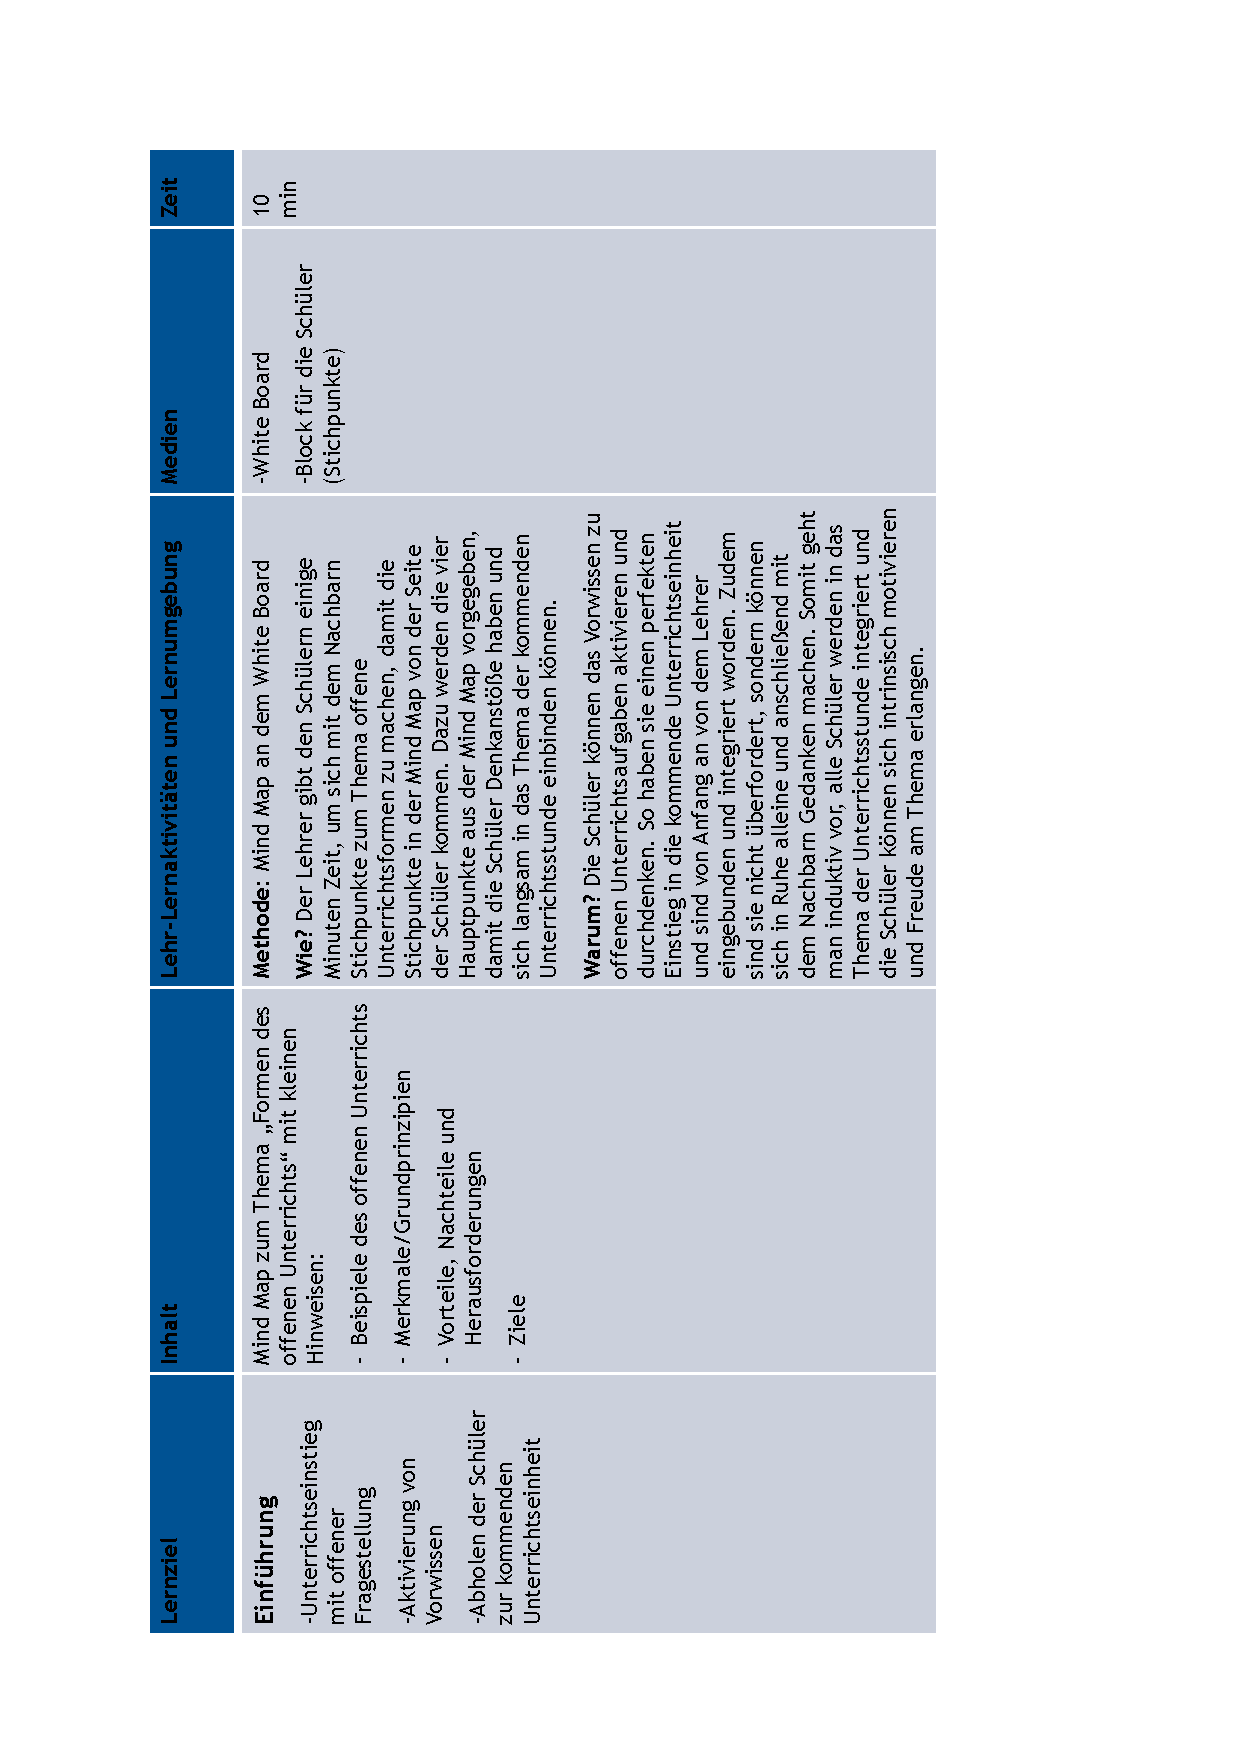
\includepdf[pages=-]{unterrichtsplanung}

\end{document}
